\section{Data Description}

\subsection{Data Collection}

The data about \textcolor{blue}{Detroit River} used in this program is provided by Professor Jan and
 was originally collected by Jian and her team during the Lake Huron–Lake Erie Corridor survey in July-August 2004.
  The survey collected 16 taxonomic variables, 8 environmental 
  variables, and 30 stressors across the study zone.

% \textcolor{blue}{(the places been surveyed)}

The sampling site locations were determined prior to 
fieldwork by a stratified random sampling design to ensure representative coverage. 
The sampling zone encompassed the entire Detroit River, including both the upstream mixing zone 
with Lake Saint Clair and the downstream transition into the Lake Erie entrance.

To enhance the estimation and control of temporal variability, 
data from two previous studies—which collected environmental conditions in the same survey zone 
(Farara and Burt 1993; Wood 2004)—were compiled and incorporated by Jian and her team into the 2004 data set. 
Both of these earlier data sets followed the same field protocols as the 2004 Lake Huron-Lake Erie Corridor survey.
For the taxonomic data, information from three separate benthic surveys was combined to
increase sample size and provide more details on taxonomic. 
These combinations improved environmental clustering of aquatic sites and the construction of zoobenthic community indicators. 

% The sampling sites in the Detroit River zone of the Lake Huron-Lake Erie Corridor survey 
% and the sampling places in the two previous studies are shown in Figure \ref{fig:different_data_sampling_locations}.

\begin{figure}[!h]
    \centering
    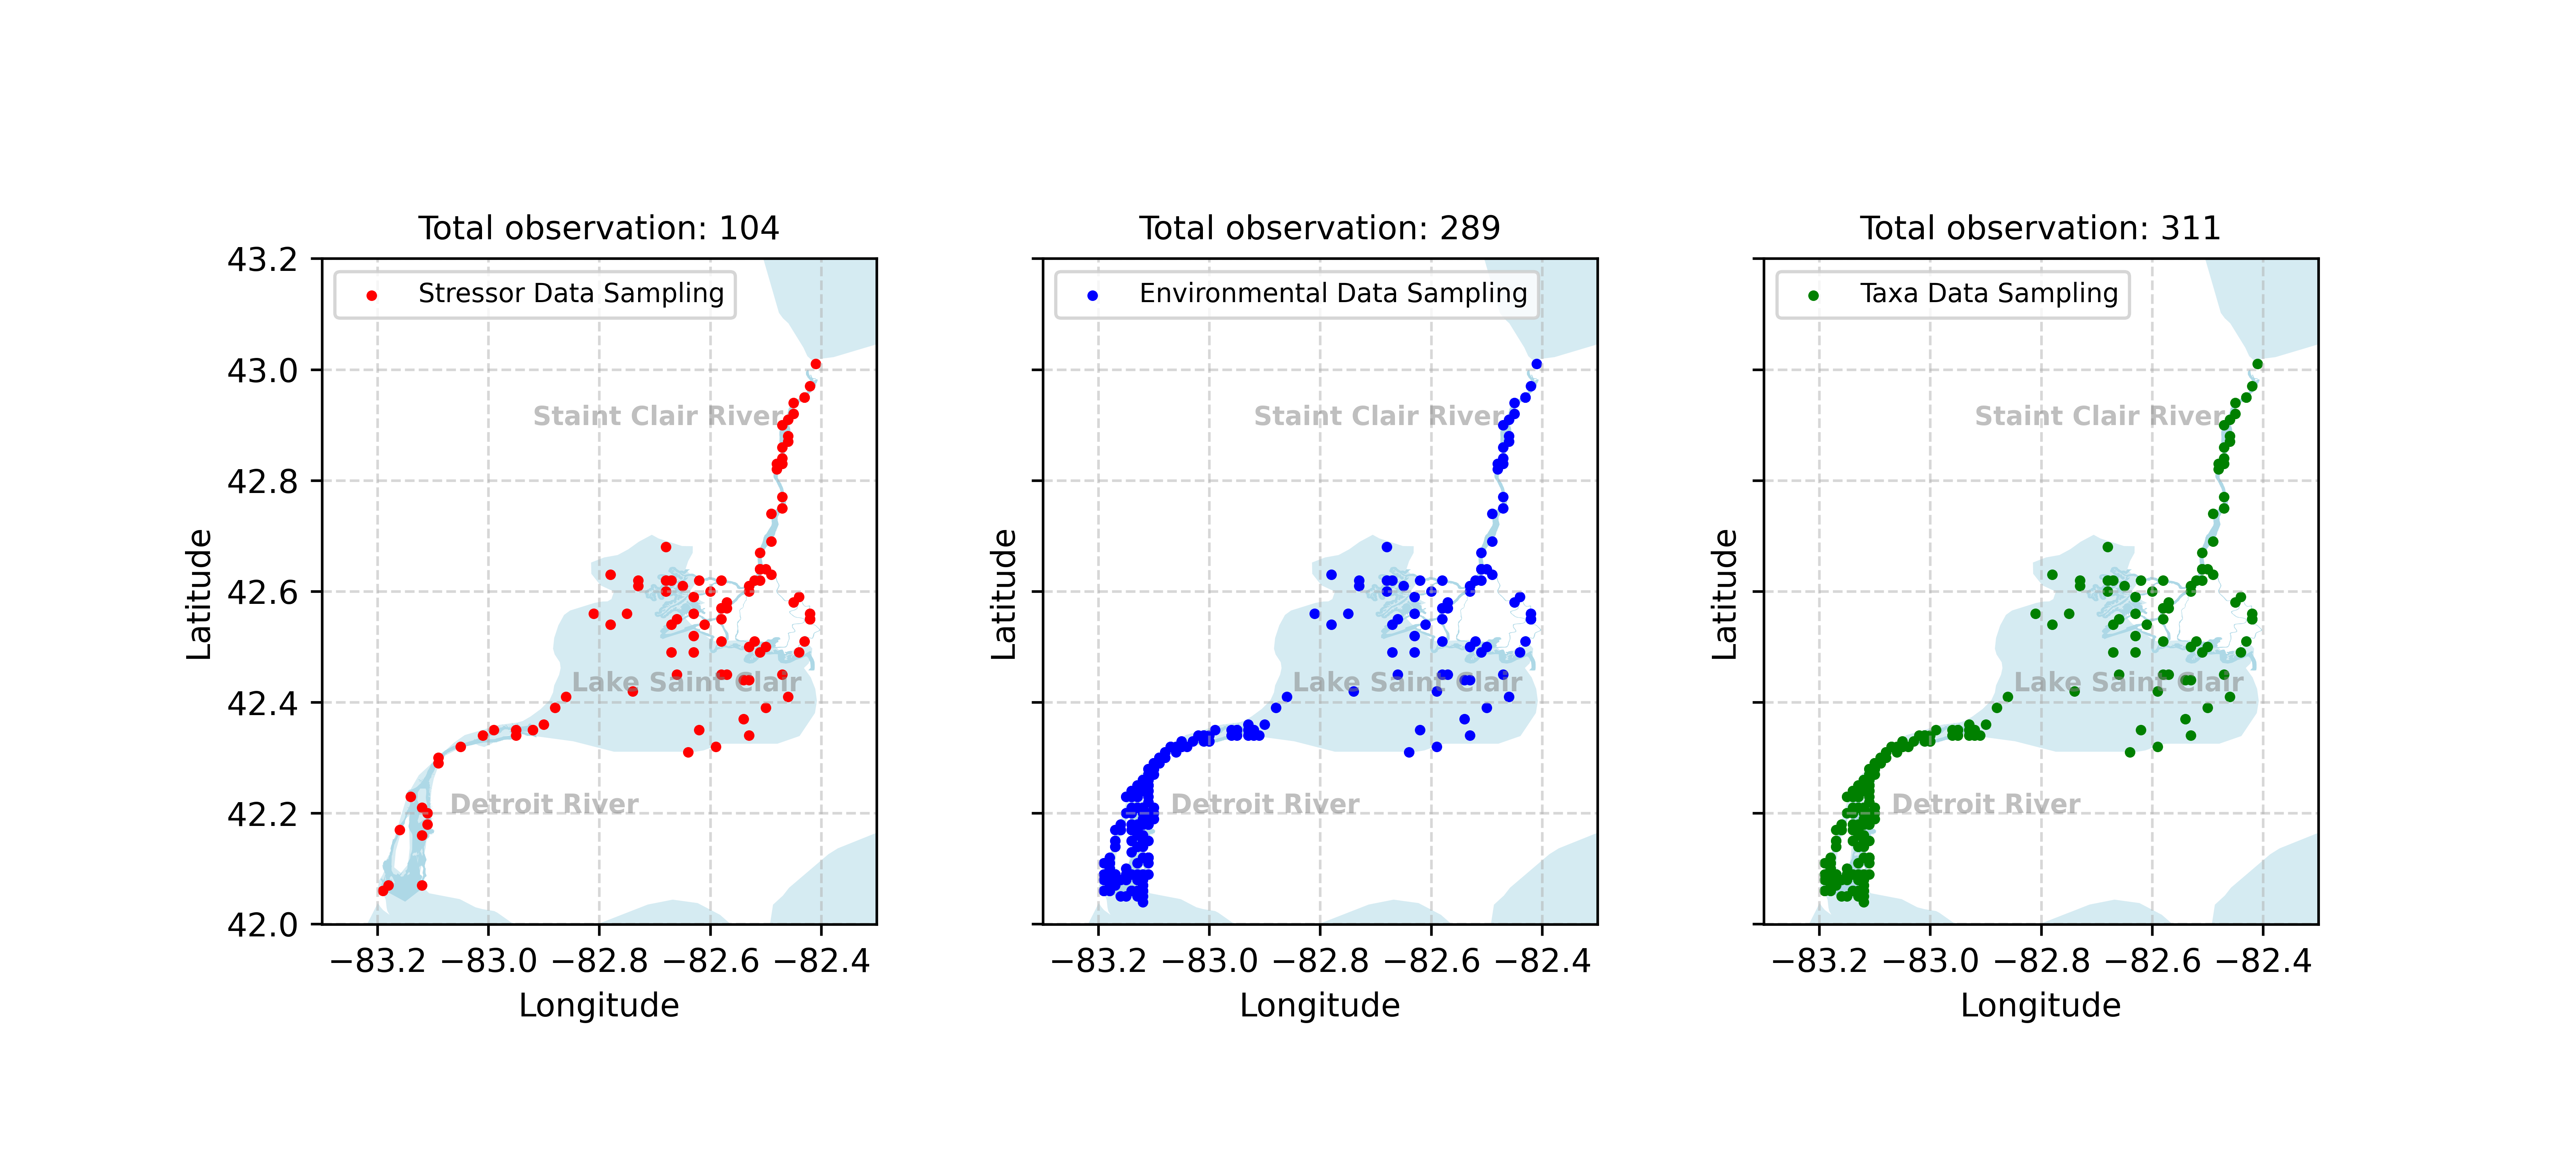
\includegraphics[width=1\textwidth]{../results/different_data_sampling_locations.png}
    \caption{Different data sampling locations of the three types of data in the Lake Huron-Lake Erie Corridor survey area.}
    \label{fig:different_data_sampling_locations}
\end{figure}

In data quality checking work, an evaluation of the sampling sites, as shown in Figure~\ref{fig:different_data_sampling_locations},
reveals a spatial mismatch in the data sources: the taxonomic, environmental, and stressor datasets are not
fully aligned across the survey area. 
\footnote{By checking the thesis page 24, data from two previous studies was incorporated and compiled, but
it did not mention what specific data type was included. Meanwhile, data from three separate benthic surveys
was also combined into the 2004 data set.}
Additionally, Figure~\ref{fig:desmonstration_of_influence_by_different_sampling_zones_and_amount}
visually illustrates how discrepancies in sampling locations and dataset sizes may affect the validity of modeling efforts. 
To address this issue, only those sites that contain all three types of data—taxonomic, environmental,
and stressor—should be used to train the model.

A further comparison with the appendix of Jian’s thesis (p.~164) shows that the
full environmental dataset includes 311 sampling sites distributed across the Detroit River, 
Lake St. Clair, and St. Clair River zones. While the current dataset in use does not include all 
these sites, this limitation can be resolved by accessing the full environmental and 
taxonomic data from Jian’s appendix and merging them by the site ID.

However, the stressor data presents a unique constraint: it is not included in the appendix 
and is only available in a separate file that contains measurements distributed across the three major zones. 
As such, this dataset reflects stressor impacts at a broader corridor scale, not limited to the Detroit River zone. 
% This complicates efforts to conduct zone-specific stress evaluations.

% \begin{tcolorbox}[colback=yellow!10!white,
%                                         colframe=blue!80!black,
%                                         title =Probelm in repeatative measurements at the same site,
%                                         fonttitle=\bfseries] 
% Because the comprehensive data(environmental and stressors) was merged from three studies conducted in 1991, 1999 and 2004,
% the sites that were sampled in the studies were not pre-determined to be the same or totally different. Therefore,
% some sites were sampled all three times, which some were sampled only once or twice, this may cause the problem of repeatative measurements at the same site.
% \textbf{However,} considering the time span of the three studies, the minimum of 5 years and maximum of 13 years, the repeatative measurements can be 
% treated as independent observations, even though they were taken at the locations. If it is not acceptable, we can go to find other appraoches to deal with it.

% Such repeatative measurements at the same site can be spoted by checking the same location(latitude and longitude) in the appendix,
% but their site IDs are different, which means the author did not consider them as different observations.
% \end{tcolorbox}

% \begin{tcolorbox}[colback=yellow!10!white,
%                                         colframe=blue!80!black,
%                                         title =Problem of not-aligned observations and differences in amount of data,
%                                         fonttitle=\bfseries] 
% After checing the appendix table in Jian's thesis (p164), which contains the full environmental data(311 sites) over three areas
% (Detroit River, Lake St Clair and St Clair River), I found that the data i currently have is not aligned with the amount of data in Jian's work.
% It is not a big problem because i can acesss the full 311 sites data of environmental and taxonomic data from the appendix and merge them by the site ID.

% \textbf{However, the stressor data is not available in the appendix}, and the stressor data i have actually spreads over the three areas (Detroit River, Lake St Clair and St Clair River),
% which means the stress evaluation from it is not limited to the Detroit River zone, but the weighted average of the evaluation from the three areas.

% This can be an issue when we want to fully evaluate the stressor impact on the Detroit River zone. \textbf{But it can also be a new viewpoint} that is to evaluate the stressor impact from a 
% broader perspective, then build the model of the taxa-stressor relationship based on these spreaded sites. Apply the fiited model on the rest sites with 
% the taxa and environmental data to predict their stressor impact, which includes the Detroit River zone.

% By following this approach, \textbf{our study area is not limited to the Detroit River zone}, but the whole sampling locations, Lake Huron-Lake Erie Corridor survey area.
% \end{tcolorbox}

% \begin{figure}[!ht]
%     \centering
%     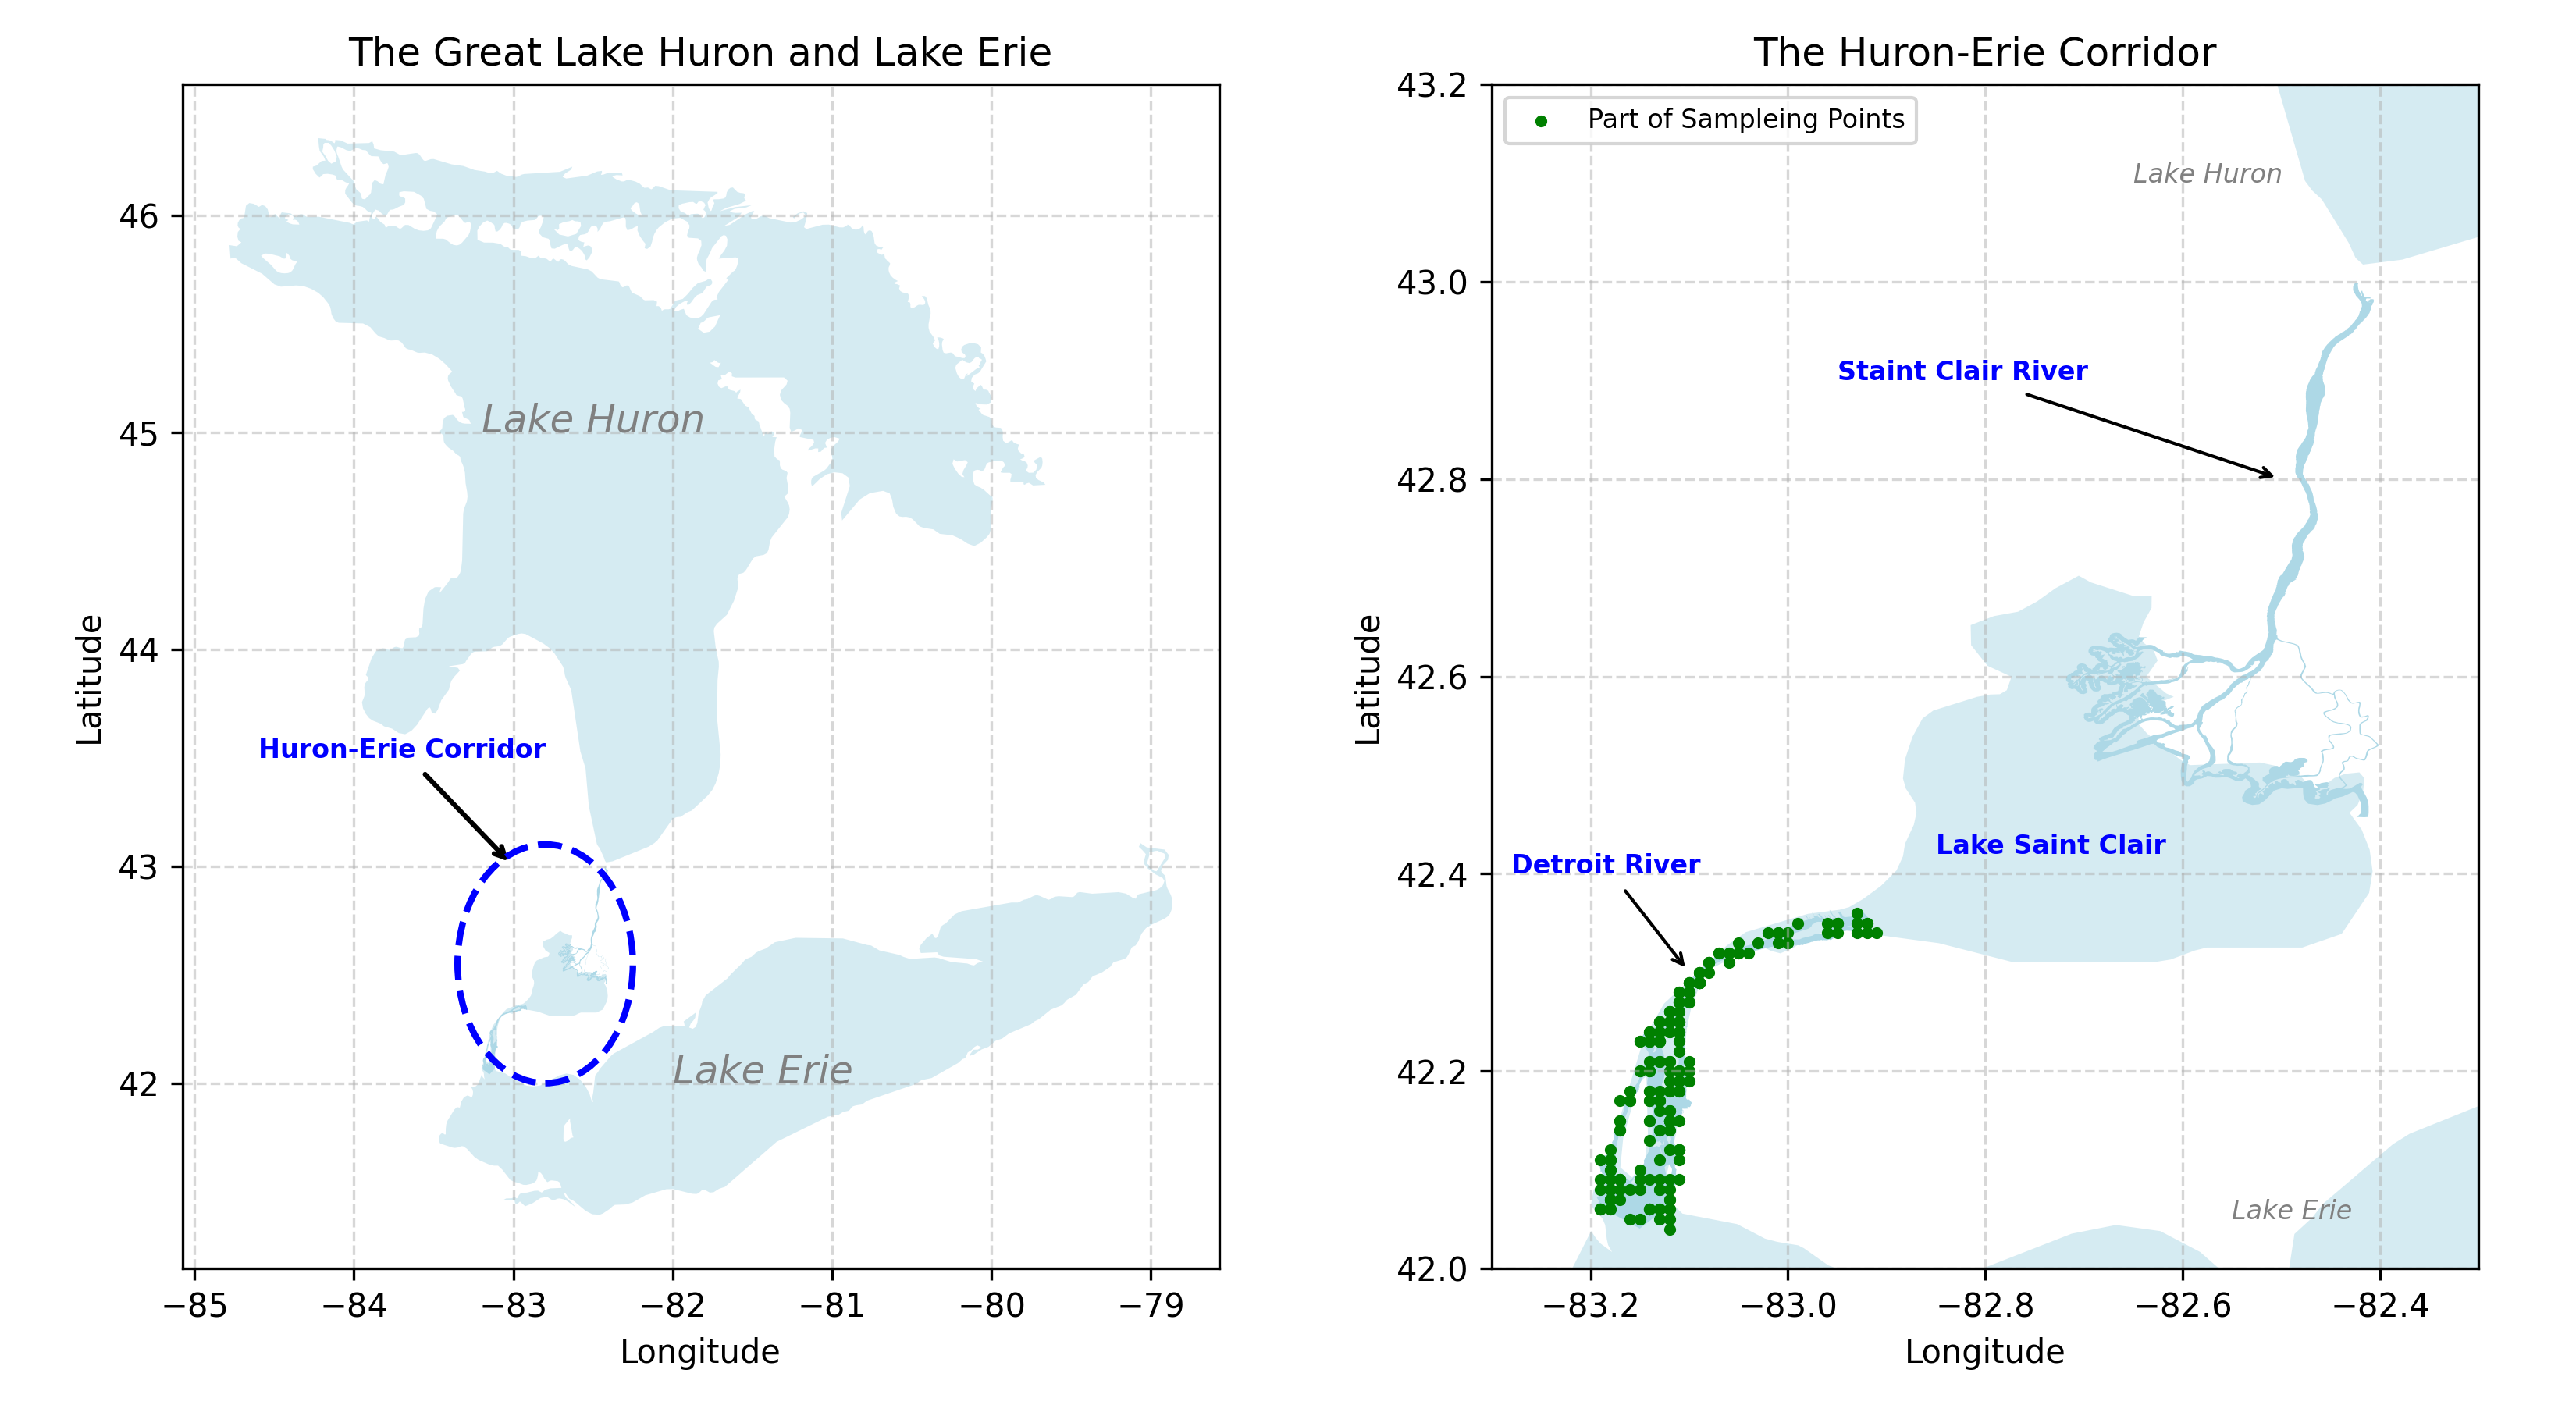
\includegraphics[width=0.9\textwidth]{../results/map_of_huron_erie_corridor.png}
%     \caption{Waiting to be updated}
%     \label{fig:map_of_huron_erie_corridor}
% \end{figure}

\subsection{Environmental attributes and samples}

In the 2004 Lake Huron-Lake Erie Corridor survey, eight environmental attributes were measured at each sampling site. The site \textbf{location} (longitude and latitude) was recorded based on the GPS reading.

\textbf{Temperature ($^\circ$C)} and \textbf{dissolved oxygen concentration ($mg/L$)} were measured with a Hydrolab multimeter. 
\textbf{Water depth ($m$)} was recorded from the Ponar rope, and \textbf{water velocity ($m/s$)} 
(measured 0.5 meters below the surface) was obtained with an Ott C-3 portable current meter. 
\textbf{Loss on ignition (\%)} and \textbf{median particle size (phi-units)} were determined during sediment 
processing but are treated as environmental attributes due to their fundamental roles in habitat
 characterization (details on their analysis are provided in a later subsection).
\footnote{Although loss on ignition and median particle size are derived from sediment samples, 
they are considered environmental variables because they reflect essential physical and chemical habitat features.}

\vspace{0.2em}
The meanings and ecological relevance of these six attributes are as follows:

\begin{itemize}
    \item \textbf{Temperature ($^\circ$C):} Water temperature affects metabolic rates, distribution, and activity patterns of aquatic organisms.
    \item \textbf{Dissolved Oxygen Concentration ($mg/L$):} Indicates the amount of oxygen available for aquatic life; low levels can limit survival and exclude sensitive taxa.
    \item \textbf{Water Depth ($m$):} Influences light penetration, stratification, and habitat availability for benthic organisms.
    \item \textbf{Water Velocity ($m/s$):} Reflects the flow regime, which shapes sediment characteristics and determines which taxa can colonize a site.
    \item \textbf{Loss on Ignition (\%):} Measures organic matter content in sediments, indicating productivity and food resource availability for benthic fauna.
    \item \textbf{Median Particle Size (phi-units):} Describes sediment texture, affecting substrate stability and the suitability of habitats for different taxa.
\end{itemize}

\vspace{0.2em}
These environmental attributes collectively characterize the abiotic conditions at each site and strongly influence the taxonomic composition and abundance of benthic invertebrate communities.

Additionally, these attributes are commonly used to describe the baseline environmental conditions of aquatic habitats, as they are primarily governed by natural physical and chemical processes. 
By including these variables as covariates in the analysis, we can better control for natural
environmental variation in the taxonomic composition of zoobenthic communities, thereby
isolating the effects of stressors of interest. However, it is important to note 
that certain attributes (e.g., organic matter content or temperature) may also be
indirectly influenced by anthropogenic activities in some settings. 
Care was taken to interpret their roles in the context of site history and
land use, but in general, these variables serve as key descriptors of the 
underlying habitat conditions independent of direct contamination or disturbance.

To ensure comparability of the merged data, the 2004 Lake Huron-Lake Erie Corridor survey followed
the same sampling protocols as those used in the two previous studies when recording environmental attributes.

\subsection{Taxonomic attributes and samples}
The zoobenthos were collected with a Petie Ponar grab sampler. 
After considering the fullness of each grap and the removing of fine materials,
the team applied multiple grabs at each site until a total volume of 2\(L\) sediment was collected.
The sediment samples for organic and metals analysis were preserved in corresponding professional containers, 
all these samples were stored frozen.

One zoobenthic sample replicate from each site was randomly selected and processed, 
while the other two were archived. Samples were sieved into size fractions (4 mm, 1 mm, 0.5 mm, 0.25 mm), 
then elutriated to separate lighter detritus and animals from inorganic sediments. 
Each fraction was sorted under a microscope and organisms were identified to the lowest 
possible taxonomic rank using standard keys. Zoobenthos were preserved in 70\% ethanol in 
labeled vials and archived at the University of Windsor.

Specifically, there were 16 taxa recorded from the sediment samples, as shown in the table \ref{tab:taxonomic_variables}.
According to their creature characteristics and preferred habitat, these taxa can be gently divided into three groups:

\begin{table}[htbp]
\centering
\caption{Benthic Taxa with Explanation and Preferred Habitat Feature}
\label{tab:taxonomic_variables}
\begin{tabular}{|>{\centering\arraybackslash}m{3cm}|>{\centering\arraybackslash}m{5cm}|>{\centering\arraybackslash}m{4cm}|}
\hline
\textbf{Taxa} & \textbf{Explanation} & \textbf{Preferred Habitat} \\
\hline
Nematoda         & Roundworms                   & \multirow{6}{*}{Broad} \\
Chironomidae     & Non-biting midges (larvae)   &  \\
Ceratopogonidae  & Biting midges                &  \\
Amphipoda        & Small crustaceans (scuds)    &  \\
Acari            & Aquatic mites                &  \\
Hydrozoa         & Small predatory animals      &  \\
Gastropoda       & Snails and slugs             &  \\
\hline
Oligochaeta      & Aquatic segmented worms      & \multirow{6}{*}{Depositional zone} \\
Hexagenia        & Mayfly genus (larvae)        &  \\
Dreissena        & Zebra/quagga mussels         &  \\
Hirudinea        & Leeches                      &  \\
Turbellaria      & Flatworms                    &  \\
Sphaeriidae      & Fingernail clams             &  \\
\hline
Caenis           & Mayfly genus (larvae)        & \multirow{3}{*}{Erosional zone} \\
Hydropsychidae   & Net-spinning caddisflies     &  \\
Other Trichoptera& Other caddisfly families     &  \\
\hline
\end{tabular}
\end{table}

Immediately after the initial sorting of samples, ten samples were randomly selected to assess the sorting efficiency. 
One sample had a sorting efficiency of 91\%,
while the remaining samples had efficiencies of 96\% or higher.

% \begin{tcolorbox}[colback=yellow!10!white,
%                                         colframe=blue!80!black,
%                                         title =What does the numbers in the quality control mean?,
%                                         fonttitle=\bfseries] 
% To assess sorting accuracy, ten samples were randomly selected after the initial sorting
% and re-examined for missed organisms. The sorting efficiency indicates the percentage 
% of target organisms recovered in the first pass. For example, a sorting efficiency 
% of 91\% means that 91\% of the organisms were found initially, and 9\% were only discovered upon re-sorting. The remaining samples had efficiencies of 96\% or greater, confirming a high level of accuracy in the sorting process.
% \end{tcolorbox}

% \textcolor{red}{why the taxa data are useful in assessing the integrity of the aquatic ecosystem?
% this part should be put into introduction or research objectives sections.}
Each taxa responses to the changs in environmental and stress conditions differently, modeling this changes-response relationship will 
help us to understand how the zoobenthic community reacts to the external changes and use their response to assess the ecological integrity.

However, to consider the precise response of each taxa to the infinite environmental and stressor changes is impossible, 
but knowing how they respond to the stressors can help identify the level of impairment that
was caused by anthropogenic activities.
An alternative way to assess the taxonomic response to the stressors is to observe the changes in taxonomic composition,
which is a generalized response of the zoobenthic community instead of the individual taxa. This generalized response is more 
representative than a single or a few taxa and partially eliminates the noise in taking limited taxa group, in which the noise may be caused by the 
subtle changes(too small to be detected) in the external conditions.

\subsection{Stressors samples}

Sediment samples from each site were thoroughly mixed to ensure homogeneity. The homogenized samples were then split into separate portions for different analyses, including median particle size, total organic carbon (TOC), organic contaminants, and metals.

\begin{itemize}
    \item \textbf{Particle Size:} Median particle size analysis was performed by sieving dried sediment through a series of sieves of decreasing mesh size. Each size fraction was weighed and described using phi units ($\phi = -\log_2 d$), where $d$ is particle size in mm.
    \item \textbf{Total Organic Carbon (TOC):} Sediment TOC(\%OC) was determined using loss on ignition (LOI). Pre-weighed, dried sediment samples were combusted at 450$^\circ$C for 24 hours, and organic carbon was determined gravimetrically by subtracting the remaining mass.
    \item \textbf{Organic Contaminants:} The concentrations of organic contaminants(including 1245-TCB, 1234-TCB, QCB, HCB, OCS, p,p'-DDe, p,p'-DDD, mirex, Heptachlor Epoxide, total PCB)
     were measured using a gas chromatograph equipped with a 63Ni electron capture detector, following standard operating procedures.
    \item \textbf{Metals:} Metal concentrations (including Al, As, Ca, Cd, Co, Cr, Cu, Fe, Mn, Ni, Pb, and Zn) were analyzed using an Inductively Coupled Plasma Optical Emission Spectrophotometer (ICP-OES). For total mercury (Hg), an atomic absorption spectrophotometer (AAS) was used with a vapor generation accessory for increased sensitivity. Liquid samples were introduced into the instrument for metal analysis.
\end{itemize}

\begin{table}[htbp]
\centering
\caption{Sediment Stressors, Explanations, and Analytical Steps}
\label{tab:stressors_steps}
\renewcommand{\arraystretch}{1.3}
\begin{tabular}{|>{\centering\arraybackslash}m{2.7cm}|>{\centering\arraybackslash}m{6.2cm}|>{\centering\arraybackslash}m{4.0cm}|}
\hline
\textbf{Measurements} & \textbf{Explanation} & \textbf{Analytical Step} \\
\hline
\multicolumn{3}{|c|}{\textbf{Metals}} \\
\hline
Al & Aluminum (trace metal) & \multirow{11}{4cm}{ICP-OES after acid extraction (Metals step)} \\
As & Arsenic (toxic element) & \\
Ca & Calcium (major element, hardness) & \\
Cd & Cadmium (toxic metal) & \\
Co & Cobalt (trace element) & \\
Cr & Chromium (trace metal) & \\
Cu & Copper (trace metal, micronutrient) & \\
Fe & Iron (major element, micronutrient) & \\
Mn & Manganese (trace element) & \\
Ni & Nickel (trace metal) & \\
Pb & Lead (toxic metal) & \\
Sb & Antimony (trace element) & \\
V & Vanadium (trace element) & \\
Zn & Zinc (trace metal, micronutrient) & \\
\hline
Hg & Mercury (highly toxic metal) & Atomic Absorption Spectrophotometry (AAS, Metals step) \\
\hline
\multicolumn{3}{|c|}{\textbf{Total Organic Carbon}} \\
\hline
\%OC & Percent organic carbon & LOI combustion at 450$^\circ$C for 24h (TOC step) \\
\hline
\multicolumn{3}{|c|}{\textbf{Organic Contaminants}} \\
\hline
1245-TCB & 1,2,4,5-Tetrachlorobenzene (organic pollutant) & \multirow{10}{4cm}{Gas Chromatography with Electron Capture Detector (GC-ECD, Organic Contaminants step)} \\
1234-TCB & 1,2,3,4-Tetrachlorobenzene (organic pollutant) & \\
QCB & Quintachlorobenzene (organic pollutant) & \\
HCB & Hexachlorobenzene (organic pollutant) & \\
OCS & Octachlorostyrene (organic pollutant) & \\
p,p'-DDE & DDT breakdown product & \\
p,p'-DDD & DDT breakdown product & \\
mirex & Organochlorine insecticide & \\
Heptachlor Epoxide & Organochlorine pesticide breakdown product & \\
total PCB & Total polychlorinated biphenyls & \\
\hline
\end{tabular}
\end{table}

Quality assurance and chemical analyses were performed in collaboration with the Great Lakes
Institute for Environmental Research (GLIER) at the University of Windsor\cite{Zhang2008}.

Among the chemical variables analyzed, not all elements serve as stressors to benthic taxa in the same way.
Major earth elements such as Al, Ca, Fe, K, Mg, and Na are generally considered non-toxic at typical 
environmental concentrations, as they are naturally abundant in sediments and primarily reflect the 
natural composition of the substrate. However, industrial pollution or other aquatic activities 
can elevate their concentrations, making them potential stressors, though their impacts are more 
challenging to assess due to naturally high background levels.

In contrast, trace metals—including As, Bi, Cd, Co, Cr, Cu, Hg, Mn, Ni, Pb, Sb, V, and 
Zn—are regarded as pollutants due to their anthropogenic origins and toxicological effects
on aquatic organisms. Elevated concentrations of these metals usually indicate the overexploitation 
of natural resources and industrial activities, which can cause bioaccumulation and toxicity in benthic organisms. 
These metals are not biodegradable and ultimately accumulate in sediments, reflecting not only current 
but also historical pollution legacies.

Additionally, persistent organic pollutants such as PCBs, QCB, HCB, OCS, p,p'-DDE, p,p'-DDD, mirex, and
Heptachlor Epoxide originate mainly from historical industrial activities and pesticide use.
Due to their chemical stability, they persist in sediments and accumulate in aquatic food webs,
where they can cause chronic and sub-lethal effects—including reproductive and developmental 
toxicity—in aquatic organisms, and thus pose long-term risks to ecosystem health and biodiversity.

The percent organic carbon (\%OC) in sediments typically originates from the decomposition of
plant and animal material, as well as inputs from terrestrial runoff and aquatic primary production.
While not a pollutant itself, organic carbon plays a key role in sediment chemistry by 
influencing the binding and retention of contaminants, thereby affecting their mobility 
and bioavailability to aquatic organisms. High levels of organic carbon can thus modulate
the ecological impact of other pollutants in the sediment.

By distinguishing between natural background elements and anthropogenic pollutants,
these measurements enable a more accurate assessment of the sediment stress level and 
its ecological implications for the benthic community.


